\documentclass{article}
\usepackage{graphicx} % Required for inserting images
%\usepackage{amssymb}
%\usepackage{amsmath}
%\usepackage{amsfonts}
\usepackage{extarrows}
%\usepackage{mathtools}
%\usepackage{soul}
\tolerance=1
\emergencystretch=\maxdimen
\hyphenpenalty=10000
\hbadness=10000
\let\oldemptyset\emptyset
\usepackage[T1]{fontenc}

\author{Amnézic}
\date{S3 2027}
\title{Physique}

\begin{document}
\maketitle
\newpage
\tableofcontents
\newpage
\section{Introduction}
Champ :
\begin{quote}
    Un champ est une fonction définie dans un espace. Il est qualifié de scalaire lorsqu'on associe une valeur à chaque point de l'espace. Tout champ est défini par :
    \begin{itemize}
        \item une direction (une droite (ex : une droite reliant A à B))
        \item un sens (de A vers B ou de B vers A)
        \item une norme
        \item 3 composantes : (Ox,Oy,Oz) dans le plan cartésien
    \end{itemize}
    \begin{figure}[ht]
        \centering
        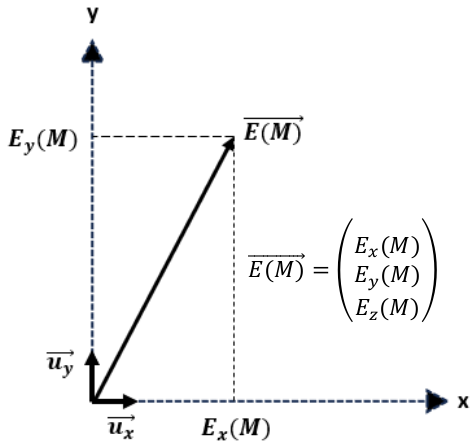
\includegraphics[scale=0.3]{figure1.png}
        \caption{Champ électrique dans un repère cartésien}
    \end{figure}
\end{quote}

Champ électrique :
\begin{quote}
    Le champ électrique $\overrightarrow{E}$ est un champ de vecteurs (dit vectoriel) qui se crée autour d'une particule M chargée (charge négative ou positive), se notant $\overrightarrow{E(M)}$.\newline
\end{quote}



Tout au long de ce chapitre, il sera nécessaire de différencier les notions suivantes :
\begin{itemize}
    \item $\overrightarrow{E(M)}$ $\rightarrow$ champ électrique
    \item ||$\overrightarrow{E(M)}$|| $\rightarrow$ norme du champ électrique (= intensité du champ au point M)
    \item E$_{x}$,E$_{y}$,E$_{z}$ $\rightarrow$ les coordonnées du champ électrique
    \item $\overrightarrow{u_{x}}$,$\overrightarrow{u_{y}}$,$\overrightarrow{u_{z}}$ $\rightarrow$ les vecteurs unitaires du repère cartésien \newpage
    \item Force et champ : une force est une interaction entre 2 particules tandis qu'un champ est un espace physique regroupant toutes les forces s'appliquant aux particules qui rentrent dans cet espace par une particule chargée
    \begin{figure}[h]
        \centering
        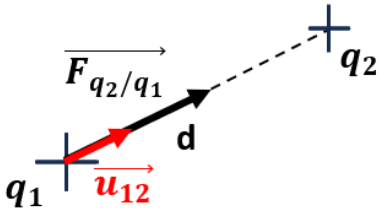
\includegraphics[scale=0.3]{figure2.png}
        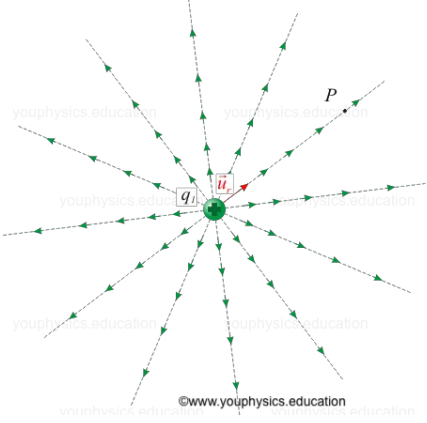
\includegraphics[scale=0.3]{figure2bis.png}
        \caption{Force électrique(gauche) et champ électrique(droite)}
    \end{figure}
\end{itemize}






\newpage
\section{Champ électrostatique créé par une distribution de charges discrètes}
\subsection{Création d'un champ électrostatique}
Une charge statique engendre autour d'elle un champ vectoriel sur tout l'espace. Le champ est constitué de l'ensemble des forces appliquées aux différents points de l'espace par la particule chargée (que l'on appelera M par convention) : il s'agit d'un champ ayant une valeur vectorielle en chaque point de l'espace \textbf{autour} du point M. Pour calculer la valeur du champ électrostatique $\overrightarrow{E(M)}$, on utilise la formule suivante :
\begin{figure}[h]
    \centering
    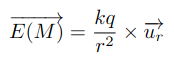
\includegraphics[scale=0.6]{firstEq.png}
    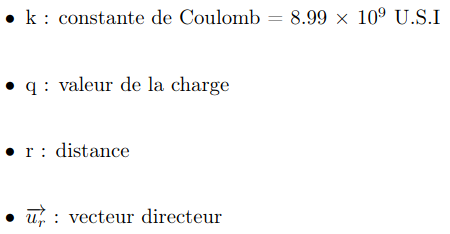
\includegraphics[scale=0.4]{values_eq1.png}
\end{figure}

Une particule "positive" engendrera un champ sortant(gauche) tandis qu'une particule "négative" engendrera un champ entrant(droite):
\begin{figure}[h]
    \centering
    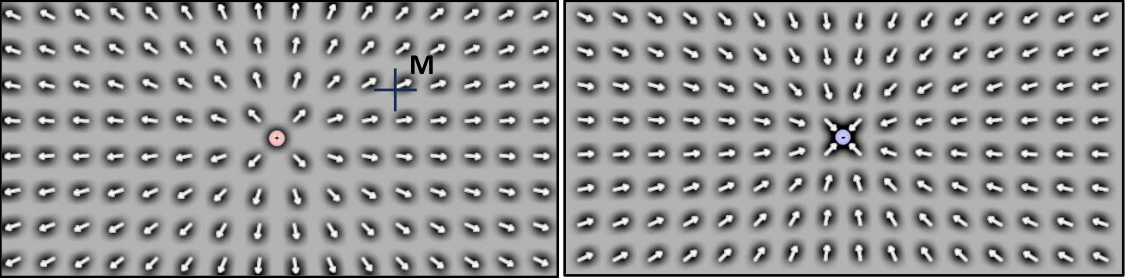
\includegraphics[scale=0.3]{champ_entrant_sortant.png}
\end{figure}

\subsection{Loi de Coulomb}



\subsection{Principe de superposition}
\subsection{Force électrique}
\end{document}